%%%%%%%%%%%%%%%%%%%%%%%%%%%%%%%%%%%%%%%%%%%%%%%%%%%
%% LaTeX book template                           %%
%% Author:  Amber Jain (http://amberj.devio.us/) %%
%% License: ISC license                          %%
%%%%%%%%%%%%%%%%%%%%%%%%%%%%%%%%%%%%%%%%%%%%%%%%%%%

\documentclass[a4paper,11pt]{book}
\usepackage[T1]{fontenc}
\usepackage[utf8]{inputenc}
\usepackage{lmodern}
%%%%%%%%%%%%%%%%%%%%%%%%%%%%%%%%%%%%%%%%%%%%%%%%%%%%%%%%%
% Source: http://en.wikibooks.org/wiki/LaTeX/Hyperlinks %
%%%%%%%%%%%%%%%%%%%%%%%%%%%%%%%%%%%%%%%%%%%%%%%%%%%%%%%%%
\usepackage{hyperref}
\usepackage{graphicx}
\usepackage{xcolor}
\usepackage{textcomp}
\usepackage[english]{babel}
\usepackage[a4paper,top=2cm,bottom=2cm,left=2cm,right=2cm]{geometry}
\usepackage{lscape}
\usepackage{caption}
\usepackage{amsmath}
\usepackage{listingsutf8}
\usepackage{listings}
\usepackage{wrapfig}
\usepackage{rotating}
\usepackage{epstopdf}
\usepackage[ruled]{algorithm2e}
\usepackage{xcolor}
\usepackage{graphics}
\usepackage{guit}

\definecolor{codegreen}{rgb}{0,0.6,0}
\definecolor{codegray}{rgb}{0.5,0.5,0.5}
\definecolor{codepurple}{rgb}{0.58,0,0.82}
\definecolor{backcolour}{rgb}{0.95,0.95,0.92}

\lstdefinestyle{mystyle}{
	backgroundcolor=\color{backcolour},   
	commentstyle=\color{codegreen},
	keywordstyle=\color{magenta},
	numberstyle=\tiny\color{codegray},
	stringstyle=\color{codepurple},
	basicstyle=\ttfamily\footnotesize,
	language = Java,
	frameround=fttt,
	frame = trBL,
	firstnumber = last,
	breakatwhitespace=false,         
	breaklines=true,                 
	captionpos=b,                    
	keepspaces=true,                 
	numbers=left,                    
	numbersep=5pt,                  
	showspaces=false,                
	showstringspaces=false,
	showtabs=false,                  
	tabsize=2
}

\lstset{style=mystyle}

\captionsetup{tableposition=top,figureposition=bottom,font=small}
%%%%%%%%%%%%%%%%%%%%%%%%%%%%%%%%%%%%%%%%%%%%%%%%%%%%%%%%%%%%%%%%%%%%%%%%%%%%%%%%
% 'dedication' environment: To add a dedication paragraph at the start of book %
% Source: http://www.tug.org/pipermail/texhax/2010-June/015184.html            %
%%%%%%%%%%%%%%%%%%%%%%%%%%%%%%%%%%%%%%%%%%%%%%%%%%%%%%%%%%%%%%%%%%%%%%%%%%%%%%%%
\newenvironment{dedication}
{
   \cleardoublepage
   \thispagestyle{empty}
   \vspace*{\stretch{1}}
   \hfill\begin{minipage}[t]{0.66\textwidth}
   \raggedright
}
{
   \end{minipage}
   \vspace*{\stretch{3}}
   \clearpage
}

%%%%%%%%%%%%%%%%%%%%%%%%%%%%%%%%%%%%%%%%%%%%%%%%
% Chapter quote at the start of chapter        %
% Source: http://tex.stackexchange.com/a/53380 %
%%%%%%%%%%%%%%%%%%%%%%%%%%%%%%%%%%%%%%%%%%%%%%%%
\makeatletter
\renewcommand{\@chapapp}{}% Not necessary...
\newenvironment{chapquote}[2][2em]
  {\setlength{\@tempdima}{#1}%
   \def\chapquote@author{#2}%
   \parshape 1 \@tempdima \dimexpr\textwidth-2\@tempdima\relax%
   \itshape}
  {\par\normalfont\hfill--\ \chapquote@author\hspace*{\@tempdima}\par\bigskip}
\makeatother

%%%%%%%%%%%%%%%%%%%%%%%%%%%%%%%%%%%%%%%%%%%%%%%%%%%
% First page of book which contains 'stuff' like: %
%  - Book title, subtitle                         %
%  - Book author name                             %
%%%%%%%%%%%%%%%%%%%%%%%%%%%%%%%%%%%%%%%%%%%%%%%%%%%

% Book's title and subtitle
\title{
	
\includegraphics[width=0.7\textwidth]{image/UniBg.png}
	\\ \Huge \textbf{Tecniche di classificazione per il riconoscimento di un tumore al cervello} \\ \huge \textit{\textbf{Documentazione progettuale}} \\ \bigskip \huge Progetto del corso di Intelligenza Artificiale\\ Università degli Studi di Bergamo}
% Author
\author{\textsc{Del Prete Giovanni - 1035205}}

\begin{document}
	\maketitle
	\thispagestyle{empty}
	\mainmatter
	\chapter{Introduzione}
	In questo documento si espone il progetto sviluppato dal sottoscritto per il corso di Intelligenza Artificiale presso l'Università degli Studi di Bergamo.
Il progetto consiste nel confrontare diverse tecniche di classificazione binaria di immagini provenienti da diverse TAC al cervello per il riconoscimento di un tumore.\\
Si ha a disposizione un dataset in formato csv che racchiude le caratteristiche dimensionali e statistiche delle immagini raccolte dalle TAC.\\

\begin{figure}[!htb]
	\minipage{0.24\textwidth}
	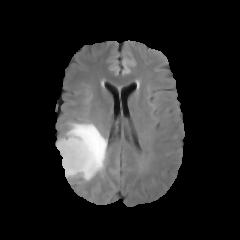
\includegraphics[width=\linewidth]{image/Image1.jpg}
	\label{fig:immagine01}
	\endminipage\hfill
	\minipage{0.24\textwidth}
	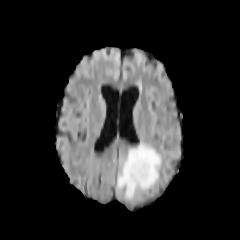
\includegraphics[width=\linewidth]{image/Image2.jpg}
	\label{fig:immagine2}
	\endminipage\hfill
	\minipage{0.24\textwidth}
	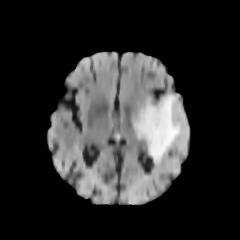
\includegraphics[width=\linewidth]{image/Image3.jpg}
	\label{fig:immagine3}
	\endminipage\hfill
	\minipage{0.24\textwidth}%
	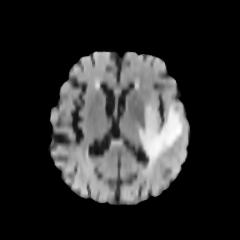
\includegraphics[width=\linewidth]{image/Image4.jpg}
	\label{fig:immagine04}
	\endminipage
	\caption{Esempio di quattro TAC al cervello}
\end{figure}

Il file \textit{bt\_dataset\_t3.csv}, disponibile sul sito \textit{www.kaggle.com}, contiene le seguenti colonne (feature):
\begin{itemize}
	\item Nome dell'immagine (ImageX, dove X indica il numero della TAC)
	\item Valori di target (1 se è un tumore, 0 se non è un tumore)
	\item Media
	\item Varianza
	\item Deviazione Standard
	\item Skewness
	\item Curtosi
	\item Contrasto (intensità)
	\item Energia
	\item ASM (Angular Second Moment), ovvero un indice che rappresenta l'uniformità del livello di grigio nell'immagine
	\item Entropia
	\item Omogeneità
	\item Dissimilarità
	\item Correlazione
	\item Ruvidezza dell'immagine
\end{itemize}
In pratica le macchie presenti nelle TAC al cervello vengono studiate come distribuzioni statistiche estrapolate da analisi di immagini.\\
L'obiettivo è quindi utilizzare le tecniche KNN, Regressione Logistica, Kernel SVM e Multi-Layer Perceptron per riconoscere quali macchie possono essere considerate tumori e quali no.\\
Gli strumenti utilizzati sono diversi moduli Python, come \textit{Pandas}, \textit{Scikit-Learn} e \textit{Matplotlib}.\\
Le diverse tecniche son state implementate in quattro file di estensione .py per facilità di lettura. In questo documento si illustreranno i punti chiave dei codici.\\
Prima di procedere con l'implementazione delle tecniche di classificazione qui sopra indicate, è stato necessario fare \textit{preprocessing} sul dataset in quanto vi sono colonne non utili (come il nome delle immagini) e alcuni dati NaN e infiniti che non sono compatibili con gli algoritmi.
	\chapter{Data Preprocessing}
	Il dataset è formato da numeri in formato float, ma in alcuni casi si hanno dei NaN o dei \textit{inf}. Occorre quindi sistemare il dataset.\\
\begin{lstlisting}
brain_tumor_data = pd.read_csv(r"Data/bt_dataset_t3.csv")

del brain_tumor_data["Image"]
brain_tumor_data = brain_tumor_data.replace(np.inf, 999)
bt_rep = brain_tumor_data.mean()
brain_tumor_data = brain_tumor_data.fillna(bt_rep)

brain_tumor_data.to_csv(r"Data/bt_dataset_t3_fixed.csv")
\end{lstlisting}

Mediante il modulo Pandas si va a leggere il file csv che costituisce il dataset e lo si trasforma in un \textit{dataframe}, in modo da poter eseguire le operazioni di preprocessing. La trasformazione in dataframe verrà eseguita in ogni algoritmo per poter eseguire le tecniche di classificazione.\\
Per i dati inf indicano un valori che tendono a infinito. Per mantenere la loro caratteristica si è pensato di sostituire i dati di tipo inf con un valore molto alto, ad esempio 999.
\begin{lstlisting}
brain_tumor_data = brain_tumor_data.replace(np.inf, 999)
\end{lstlisting}
I dati NaN sono dati che non si hanno in possesso. L'idea è quindi quella di renderli influenti negli algoritmi, perciò può essere una buona idea sostituirli con la media della colonna (feature).
\begin{lstlisting}
bt_rep = brain_tumor_data.mean()
\end{lstlisting}
Infine con l'istruzione di Pandas \textit{to\_csv()} si salvano tali operazioni in un nuovo csv che costituirà il dataset aggiustato. Il nuovo csv verrà utilizzato come input negli algoritmi che implementano le tecniche di classificazione. In questo modo si evitano errori legati all'inconsistenza dei dati.
\begin{figure}[!htb]
	\minipage{0.45\textwidth}
	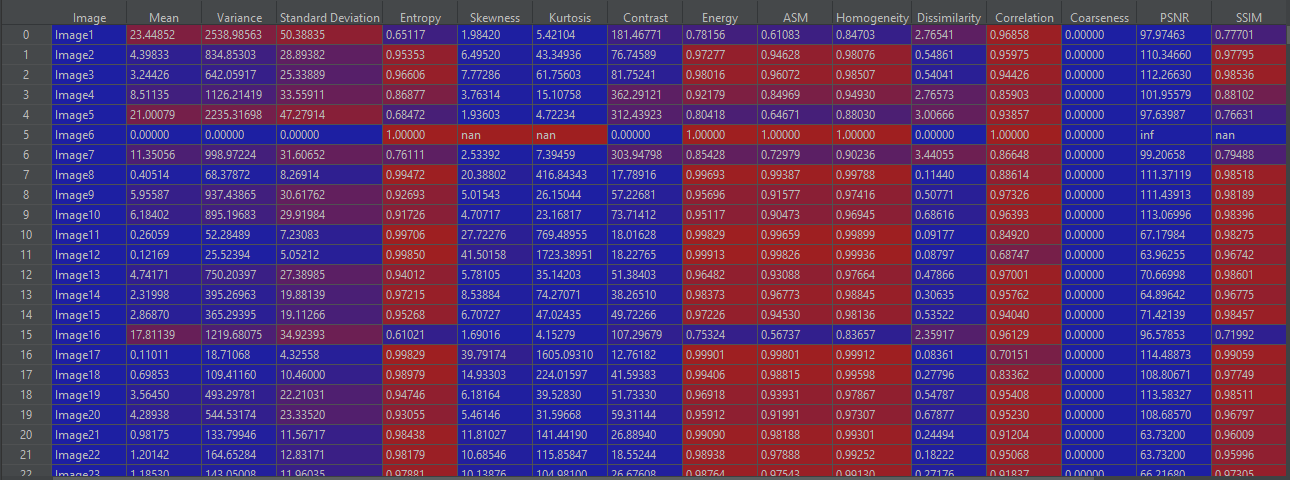
\includegraphics[width=1.2\linewidth]{image/braintumordataset.png}
	\label{fig:immagine01}
	\endminipage\hfill
	\minipage{0.45\textwidth}
	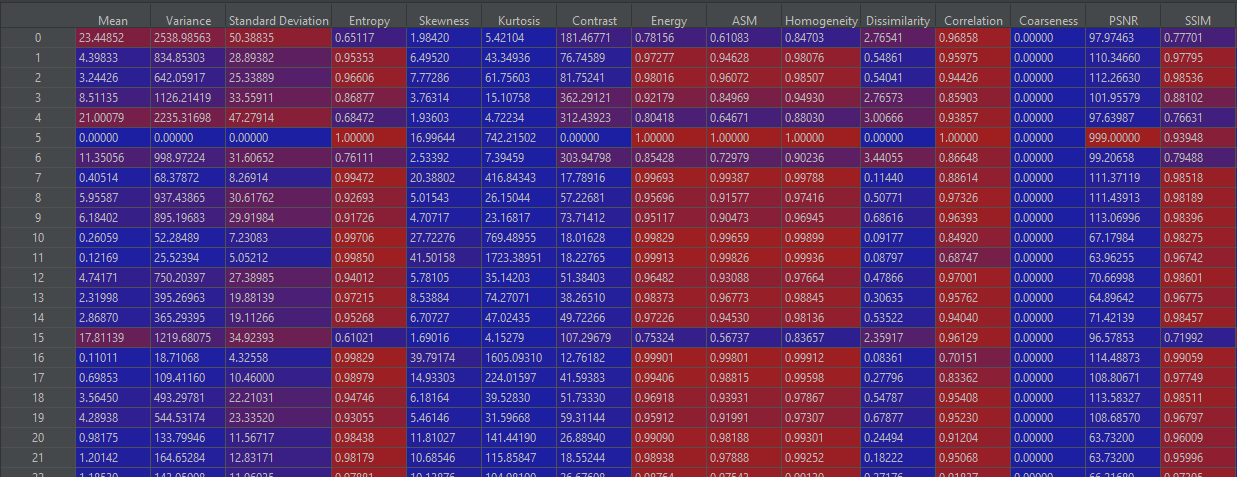
\includegraphics[width=1.2\linewidth]{image/braintumordatasetfixed.png}
	\label{fig:immagine2}
	\endminipage
	\caption{A sinistra il dataframe con dati inconsistenti, a desta il dataframe fixato.}
\end{figure}
\newpage
L'IDE utilizzato è \textit{PyCharm} e grazie al suo comodo strumento di debugging è stato semplice visualizzare la struttura del dataframe e quindi valutare il corretto funzionamento del codice. 
	\chapter{Regressione Logistica}
	\section{Regressione Logistica con tutte le feature}
La prima tecnica implementata per la classificazione binaria è la \textit{Regressione Logistica}.\\
Come accennato nei capitoli precedenti, l'obiettivo è quello di creare un modello in grado di riconoscere quando un immagine rappresenta un tumore al cervello oppure no con le migliori prestazioni possibili.\\
L'obiettivo di tale tecnica è quella di trovare il \textit{decision boundary} che suddivida nel modo più corretto possibile i target nella classe positiva (1 = è un tumore) e nella classe negativa (0 = non è un tumore).\\
Il primo passo, oltre a quello di leggere il file csv fixato e convertirlo in dataset con Pandas, è quello di portare tutti i dati nella stessa scala di valori. Ciò è utile perchè si hanno dei range di valori molto diversi e l'algoritmo potrebbe dare più importanza ai dati con range più grande. Per questo motivo si è utilizzata la classe di scikit-learn \textit{StandardScaler}. Tale classe permette semplicemente di standardizzare il dataset, ovvero portare tutti i dati in una distribuzione con media 0 e varianza 1. Perciò applicando il modello StandardScaler sui dati si ottiene un dataset con tutti i dati nella stessa scala.\\
Dal dataset occorre estrarre i \textit{regressori} (matrice X) e i \textit{target} (vettore Y). La standardizzazione ovviamente viene applicata alla matrice X.\\
\begin{lstlisting}
from sklearn.preprocessing import StandardScaler
from sklearn.model_selection import train_test_split

X = brain_tumor_data.drop("Target", axis=1).values
Y = brain_tumor_data["Target"].values
ss = StandardScaler()
X = ss.fit_transform(X)

X_train, X_test, Y_train, Y_test = train_test_split(X, Y, test_size=0.3)
\end{lstlisting}
Per la validazione del modello si sa che è necessario avere dei dati per il \textit{training} del modello e per il test. Si è ricorso quindi al metodo \textit{train\_test\_split} di scikit-learn che applica tale divisione. Si è scelto di utilizzare il 70\% dei dati per la fase di training e il 30\% per la fase di test.\\
\begin{figure}[h]
	\centering   	
	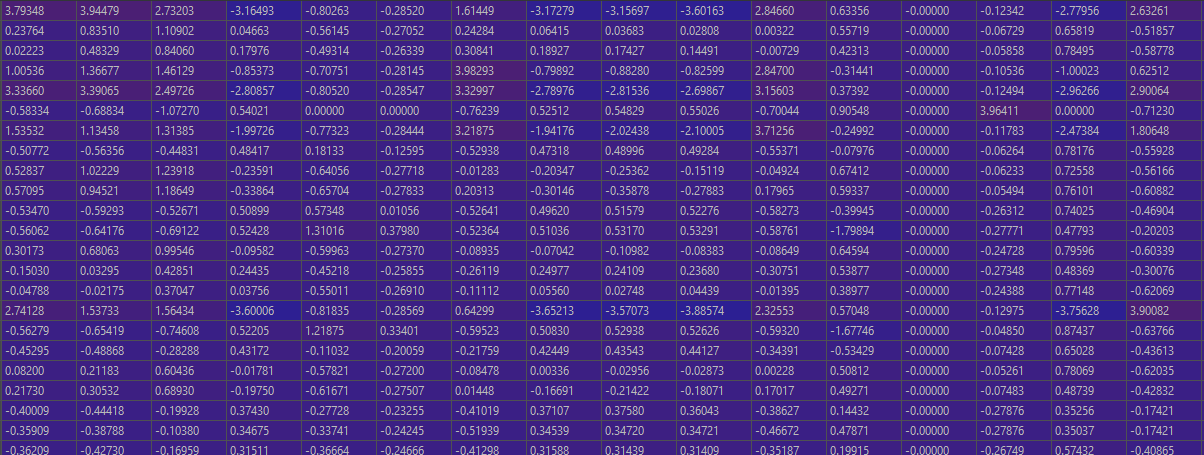
\includegraphics[width=140mm]{image/standardX.png}
	\caption{una parte della matrice X standardizzata}
\end{figure}
A questo punto si costruisce il modello di Regressione Logistica. Per farlo si utilizza la classe \textit{LogisticRegression} di scikit-learn.
\begin{lstlisting}
from sklearn.linear_model import LogisticRegression
from sklearn.metrics import accuracy_score, log_loss

log_reg = LogisticRegression()
log_reg.fit(X_train, Y_train)
Y_pred = log_reg.predict(X_test)
Y_pred_prob = log_reg.predict_proba(X_test)

acc = accuracy_score(Y_test, Y_pred)
log_loss_score = log_loss(Y_test, Y_pred_prob)
\end{lstlisting}
Con il metodo \text{fit()} di LogisticRegression si esegue la fase di training e, ovviamente, in input al metodo si passano i dati di train generati dal metodo \textit{train\_test\_split}.\\
Per valutare la bontà del modello si calcolano l' \textit{accuracy} (o accuratezza) e la \textit{Negative Log-likelihood} (o \textit{log loss}). L'accuracy è un indice che va da 0 a 1 che conta quante classificazioni son state fatte correttamente, mentre la log loss tiene conto della probabilità di appartenenza ad una determinata classe. Si punta ad avere un accuracy più alta possibile e una log loss più bassa possibile.

\section{Regressione Logistica con Dimensionality Reduction}
Il dataset è formato da 17 feature. Può essere una buona mossa applicare una tecnica di Dimensionality Reduction per poi fare classificazione? \\
Per capirlo si è utilizzata la tecnica \textit{PCA} in 2D, 3D e di dimensione tale da spiegare almeno il 95\% di varianza dei dati.
\begin{lstlisting}
from sklearn.decomposition import PCA

pca = PCA(n_components=2)
principal_components = pca.fit_transform(X)
principalDF = pd.DataFrame(data=principal_components,
columns=['principal component 1', 'principal component 2'])

finalDf = pd.concat([principalDF, brain_tumor_data[['Target']]], axis=1)

X = finalDf.drop("Target", axis=1)
Y = finalDf["Target"].values

X_train, X_test, Y_train, Y_test = train_test_split(X, Y, test_size=0.3)
\end{lstlisting}
Si è utilizzata la classe \textit{PCA} di scikit-learn. Tale classe, applicando il metodo \textit{fit\_transform()} sulla matrice X, seleziona le componenti principali (2 nel caso di PCA 2D e 3 nel caso di PCA 3D) in una matrice. Per utilizzare i dati nella tecnica di Regressione Logistica è necessario averli in formato dataframe, perciò mediante i metodi di Pandas \textit{DataFrame()} e \textit{concat()} si è costruito il nuovo dataframe con le sole componenti principali. Dopodiché si suddividono i dati di training e di test e si applica la Regressione Logistica nello stesso modo in cui è stato applicato nella sezione precedente.\\
Uno degli scopi della tecnica PCA è quella della \textit{Data Visualization}. Infatti per le tecniche di PCA in 2D e 3D vi sono porzioni di codice per la proiezione dei dati in 2D e 3D.
Per la rappresentazione in 2D è sufficiente costruire uno scatter dove negli assi vi sono le due componenti principali. I target rappresentati possono essere rossi se il valore è 1 (cioè è un tumore) e verdi se il valore è 0 (non è un tumore).
\newpage
\begin{lstlisting}
fig = plt.figure(figsize=(8, 8))
ax = fig.add_subplot(1, 1, 1)
ax.set_xlabel('Principal Component 1', fontsize=15)
ax.set_ylabel('Principal Component 2', fontsize=15)
ax.set_title('2 Component PCA', fontsize=20)


targets = [1, 0]
colors = ['r', 'g']
for target, color in zip(targets, colors):
indicesToKeep = finalDf['Target'] == target
ax.scatter(finalDf.loc[indicesToKeep, 'principal component 1']
, finalDf.loc[indicesToKeep, 'principal component 2']
, c=color
, s=50)
ax.legend(targets)
ax.grid()
plt.show()
\end{lstlisting}
Il risultato è il seguente:\\
\begin{figure}[h]
	\centering   	
	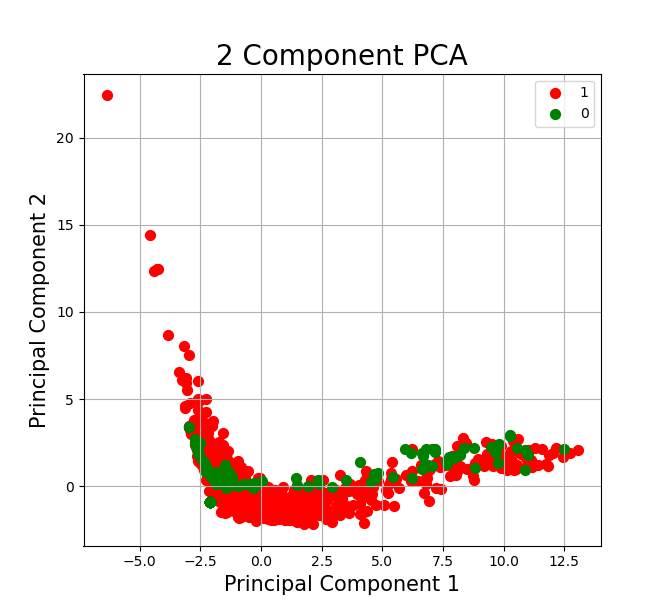
\includegraphics[width=100mm]{image/scatter2d.png}
\end{figure}
\\Per quanto riguarda la Data Visualization in 3D si utilizza la classe \textit{Axes3D} del modulo \textit{mpl\_toolkits}. La classe Axes3D permette di costruire un diagramma cartesiano con tre assi. Sui tre assi si hanno le tre componenti principali.\\
L'idea di base è quella di costruire uno scatter (come nel caso precedente) di tre dimensioni mediante matplotlib e passarlo in input alla classe Axes3D che permette la rappresentazione cartesiana.
\begin{lstlisting}
from mpl_toolkits.mplot3d import Axes3D

fig = plt.figure()
finalDf['Target'] = pd.Categorical(finalDf['Target'])
my_color = finalDf['Target'].cat.codes
ax = Axes3D(fig)
ax.scatter(finalDf['PCA1'], finalDf['PCA2'], finalDf['PCA3'], c=my_color, cmap="Set2_r", s=60)

xAxisLine = ((min(finalDf['PCA1']), max(finalDf['PCA1'])), (0, 0), (0, 0))
ax.plot(xAxisLine[0], xAxisLine[1], xAxisLine[2], 'r')
yAxisLine = ((0, 0), (min(finalDf['PCA2']), max(finalDf['PCA2'])), (0, 0))
ax.plot(yAxisLine[0], yAxisLine[1], yAxisLine[2], 'r')
zAxisLine = ((0, 0), (0, 0), (min(finalDf['PCA3']), max(finalDf['PCA3'])))
ax.plot(zAxisLine[0], zAxisLine[1], zAxisLine[2], 'r')

ax.set_xlabel("PC1")
ax.set_ylabel("PC2")
ax.set_zlabel("PC3")
ax.set_title("PCA on the iris data set")
plt.show()
\end{lstlisting}
Il risultato è il seguente:\\
\begin{figure}[h]
	\centering   	
	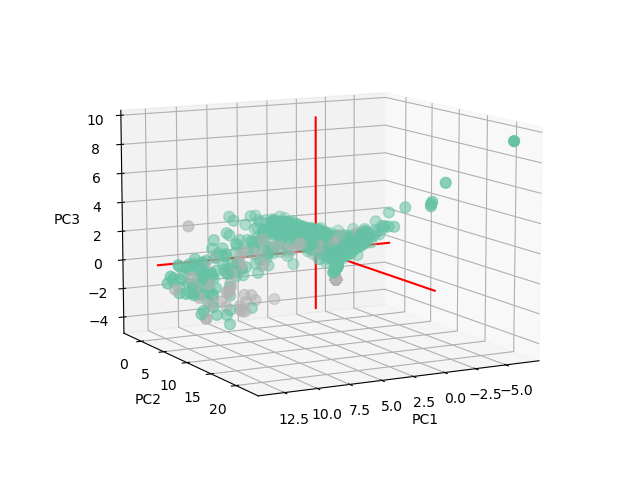
\includegraphics[width=100mm]{image/grafico3d.png}
\end{figure}

\section{Conclusione sulla Regressione Logistica}
La regressione logistica utilizzando tutte le feature è quella che dà i risultati migliori, sia in termini di accuracy e di log loss.\\
Per quanto riguarda l'utilizzo della tecnica PCA, il risultato migliore è dato dalla PCA con parametro il 95\% di varianza spiegata. In particolare, applicando dimensionality reduction a due dimensioni con PCA 2D ha peggiorato le prestazioni del modello. Ciò era intuibile guardando il grafico in due dimensioni, dove è difficile trovare un decision boundary lineare che suddivida la classe negativa con quella positiva. La situazione migliora di molto nel caso di PCA 3D, dove le prestazioni sono di poco peggiori a quelle di Regressione Logistica con PCA 95\%.
\begin{figure}[h]
	\centering   	
	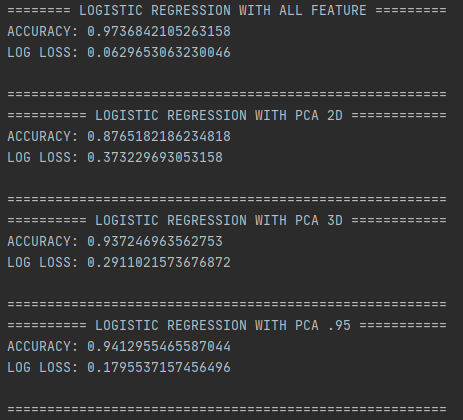
\includegraphics[width=60mm]{image/regressionelogisticaresults.png}
	\caption{Visualizzazione dei risultati stampati sulla console Python.}
\end{figure}
	\chapter{K-Nearest Neighbors}
	Un'altra tecnica implementata per il problema di classificazione delle immagini delle TAC al cervello è il \textit{K-Nearest Neighbor}. A differenza della Regressione Logistica, KNN si basa sulla classificazione con decision boundary non lineare.\\
In particolare è importante capire quanti vicini considerare nel modello, ovvero per quale K si ottiene un risultato migliore.
La classe di scikit-learn che permette di implementare l'algoritmo KNN è \textit{KNeighborsClassifier}. Tale classe ha come campo principale il campo \textit{n\_neighbors} che dà possibilità di settare il K dell'algoritmo. Di default il K è pari a 5.
\begin{lstlisting}
from sklearn.neighbors import KNeighborsClassifier

X = brain_tumor_data.drop("Target", axis=1).values
Y = brain_tumor_data["Target"].values
ss = StandardScaler()
X = ss.fit_transform(X)

X_train, X_test, Y_train, Y_test = train_test_split(X, Y, test_size=0.3)

knn = KNeighborsClassifier()
knn.fit(X_train, Y_train)

Y_pred = knn.predict(X_test)
Y_prob = knn.predict_proba(X_test)

acc = accuracy_score(Y_test, Y_pred)
log_loss_score = log_loss(Y_test, Y_prob)

print("ACCURACY: " + str(acc) + "\n")
print("LOG LOSS: " + str(log_loss_score) + "\n")
\end{lstlisting}
Il primo tentativo è quello di effettuare la classificazione KNN con K pari al valore di default, ovvero 5. Si ha un accuracy pari a circa 0.95, mentre il log loss è pari a 0.5 e quindi abbastanza alto.\\
A questo punto si vuole verificare per quale K si ha il risultato migliore in termini di accuracy e log loss. Per fare ciò si implementano più modelli per più K e si visualizzano le metriche su grafici per valutare per quali K il modello ha le migliori prestazioni.\\
L'idea è quella di utilizzare un ciclo for per costruire un modello con K che va da 1 a 20; \textit{Ks} è un array che contiene i diversi valori di K che ad ogni iterazione viene modificato e di seguito si effettuano le fasi di train e di test. A questo punto si calcolano le metriche, ovvero l'accuracy e log loss.
\begin{lstlisting}
Ks = [1, 2, 3, 4, 5, 6, 7, 8, 10, 11, 12, 13, 14, 15, 16, 17, 18, 19, 20]
accuracys = np.array([])
scores = np.array([])
for K in Ks:
print("============ "+"K="+str(K)+" ============")
knn = KNeighborsClassifier(n_neighbors=K)
knn.fit(X_train, Y_train)

Y_pred_train = knn.predict(X_train)
Y_prob_train = knn.predict_proba(X_train)

Y_pred = knn.predict(X_test)
Y_prob = knn.predict_proba(X_test)
Y_pred = knn.predict(X_test)
Y_prob = knn.predict_proba(X_test)

acc = accuracy_score(Y_test, Y_pred)
accuracys = np.append(accuracys,acc)
log_loss_score = log_loss(Y_test, Y_prob)
scores = np.append(scores, log_loss_score)

print("ACCURACY: " + str(acc))
print("LOG LOSS: " + str(log_loss_score) + "\n")
print("===========================================")
\end{lstlisting}
Per il plotting delle metriche in funzione dei diversi K si utilizza semplicemente, ancora una volta, il modulo matplotlib di Python.\\
Nel passo precedente, ovvero nel ciclo for, si salvano le metriche in due array numpy che verranno utilizzati proprio in questo passo.
\begin{lstlisting}
x_plot = np.array(Ks)
y_plot = accuracys
y_plot_2 = scores

plt.plot(x_plot, y_plot, 'r--', label="Accuracy")
plt.xticks(np.arange(x_plot.min(), x_plot.max(), 1))
plt.legend()
plt.show()

plt.plot(x_plot, y_plot_2, 'bs', label='Log loss score')
plt.xticks(np.arange(x_plot.min(), x_plot.max(), 1))
plt.legend()
plt.show()
\end{lstlisting}
\begin{figure}[!htb]
	\minipage{0.45\textwidth}
	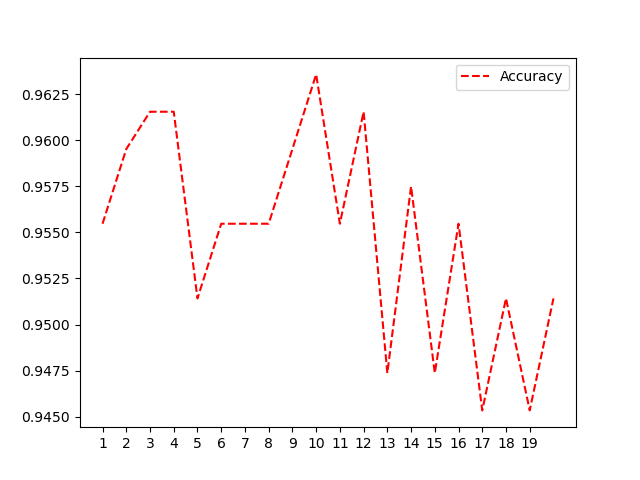
\includegraphics[width=1.2\linewidth]{image/plot_accuracy.png}
	\label{fig:immagine01}
	\endminipage\hfill
	\minipage{0.45\textwidth}
	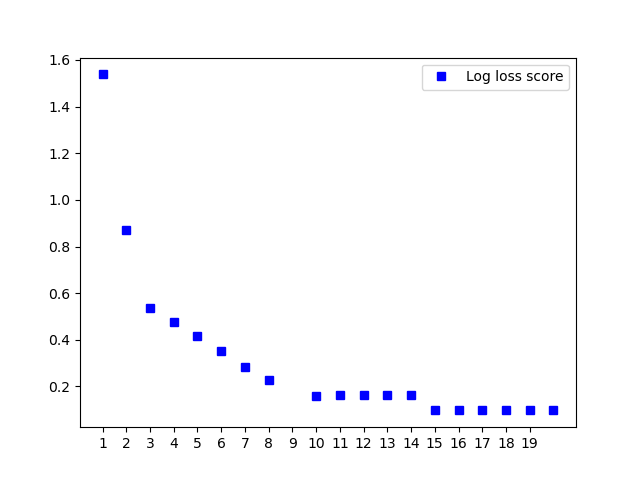
\includegraphics[width=1.2\linewidth]{image/plot_logloss.png}
	\label{fig:immagine2}
	\endminipage
	\caption{A sinistra il plot delle accuracy, a desta quello delle log loss.}
\end{figure}
In termini di accuracy i valori oscillano tra 0.94 a 0.96 con un andamento piuttosto irregolare. In qualsiasi caso, per K che va da 1 a 20 si ha un buon risultato in termini di accuracy.\\
Per quanto riguarda la log loss si nota dal grafico un andamento simile ad un ramo di iperbole. Per K molto bassi (ad es. K = 1 e K = 2) si ha log loss molto alto. All'aumentare del K si ha log loss molto più basso fino a raggiungere un valore limite pari a circa 0.1 per K > 15.
\section{Conclusioni finali sul KNN}
Dal punto di vista dell'accuracy utilizzare un K basso o alto non comporta grosse differenze. Il grafico della log loss suggerisce di utilizzare un K alto in quanto si ha un legame decrescente al crescere di K fino a raggiungere il valore limite.\\
Un buon valore di K per ottenere un ottimo trade off tra accuracy e log loss è 17 (accuracy = 0.96 e logloss = 0.1).
	\chapter{Kernel SVM}
	In questo capitolo si mostra la classificazione mediante \textit{SVM} con kernel trick.\\
Anceh in questo caso si utilizzano le tecniche di PCA per la dimensionality reduction, come nel caso della regressione logistica.\\
I kernel utilizzati sono quello lineare, gaussiano e la funzione sigmoide.\\
Il modello SVM è incluso nella classe \textit{SVC} di scikit-learn.\\
Un problema notato nei capitoli precedenti è che le due classi non sono molto divisibili da un decision boundary lineare. Infatti ci si aspettano prestazioni migliori utilizzando il kernel gaussiano o con la funzione sigmoide.
\begin{lstlisting}
from sklearn.svm import SVC

pca = PCA(n_components=2)

principal_components = pca.fit_transform(X)
principalDF = pd.DataFrame(data=principal_components,
columns=['principal component 1', 'principal component 2'])

finalDf = pd.concat([principalDF, brain_tumor_data[['Target']]], axis=1)

X = finalDf.drop("Target", axis=1)
Y = finalDf["Target"].values

X_train, X_test, Y_train, Y_test = train_test_split(X, Y, test_size=0.3)

svc = SVC(kernel="linear", probability=True)
svc.fit(X_train, Y_train)
score_linear2d = svc.score(X_test, Y_test)
print("=========== PCA 2D ===========")
print("ACCURACY WITH LINEAR KERNEL: " + str(score_linear2d))

svc = SVC(kernel="rbf", probability=True)
svc.fit(X_train, Y_train)
score_rbf2d = svc.score(X_test, Y_test)
print("ACCURACY WITH GAUSSIAN KERNEL: " + str(score_rbf2d))

svc = SVC(kernel="sigmoid", probability=True)
svc.fit(X_train, Y_train)
score_sigmoid2d = svc.score(X_test, Y_test)
print("ACCURACY WITH SIGMOID KERNEL: " + str(score_sigmoid2d))
\end{lstlisting}
Nella classe SVC vengono settati i campi \textit{kernel} e \textit{probability}. Il campo kernel permette di specificare quale tipo di kernel utilizzare per misurare la somiglianza tra due sample. Il campo probability viene settato a \textit{true} per includere il calcolo della probabilità di accuratezza delle predizioni. Ciò rallenta di non poco l'algoritmo ma può essere utile per avere un ulteriore feedback sulle prestazioni del modello.\\
\section{Conclusioni su classificazione con SVM}
\begin{figure}[h]
	\centering   	
	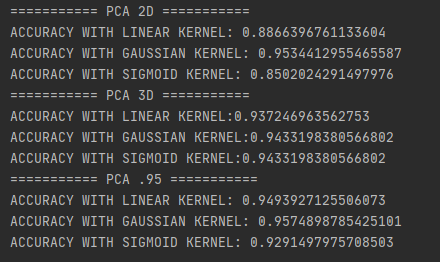
\includegraphics[width=100mm]{image/svmresults.png}
	\caption{Risultati stampati sulla console Python}
\end{figure}
Come ci si aspettava la tecnica migliore risulta quella ottenuta con kernel gaussiano e con PCA 95\%.\\
Come si può notare però, il contributo maggiore viene fornito dal tipo di kernel. Infatti per il dataset in questione il kernel più performante è quello gaussiano a prescindere dal tipo di PCA utilizzato. Infatti nei tre casi di PCA si nota che le prestazioni del modello SVM con kernel gaussiano cambiano di poco, mentre il tipo di tecnica PCA utilizzata può influire molto se si utilizzano kernel lineari o sigmoidali.
	\chapter{Classificazione con Multi-Layer Perceptron}
	In questo capitolo si utilizza una tecnica basata su rete neurale, ovvero il \textit{Multi-Layer Perceptron}.\\
Mediante scikit-learn è possibile decidere quanti hidden layer inserire e di quali dimensioni. La classe che permette di costruire un MLP è \textit{MLPClassifier}. Inoltre è possibile selezionare il tipo di funzione di attivazione nei neuroni interni:
\begin{itemize}
	\item \textit{identity}: funzione identità $f(x)=x$;
	\item \textit{logistic}: funzione sigmoide tipica della regressione logistica $f(x)=\frac{1}{1+e^{-x}}$
	\item \textit{tanh}: funzione tangente iperbolica $f(x)=\tanh(x)$
	\item \textit{relu}: funzione lineare $f(x)=\max(0,x)$
\end{itemize}
\begin{lstlisting}
from sklearn.neural_network import MLPClassifier

X = brain_tumor_data.drop("Target", axis=1).values
Y = brain_tumor_data["Target"].values
ss = StandardScaler()
X = ss.fit_transform(X)

X_train, X_test, Y_train, Y_test = train_test_split(X, Y, test_size=0.3)

mlp = MLPClassifier(hidden_layer_sizes=(100,), activation='relu', verbose=True, max_iter=300)
mlp.fit(X_train, Y_train)

y_pred_train = mlp.predict(X_train)
y_prob_train = mlp.predict_proba(X_train)

y_pred = mlp.predict(X_test)
y_prob = mlp.predict_proba(X_test)

accuracy_train = accuracy_score(Y_train, y_pred_train)

loss_train = log_loss(Y_train, y_prob_train)

print("ACCURACY: TRAIN=%.4f" % accuracy_train)
print("LOG LOSS: TRAIN=%.4f" % loss_train)
\end{lstlisting}

Il modello adottato è un MLP con un hidden layer formato da 100 neuroni e con funzione di attivazione lineare (relu). I campi \textit{verbose} e \textit{max\_iter} sono utili per la fase di addestramento della rete neurale; il primo è utile per visualizzare in maniera dinamica e testuale la fase di addestramento, mentre il secondo permette di inserire il massimo numero di iterazioni nella fase di addestramento. Sperimentalmente il massimo di 300 iterazioni sono risultati sufficienti per raggiungere l'obiettivo.\\
La fase di addestramento della rete viene iterata finchè non vi sono 10 epoche consecutive dove il loss score non diminuisce di almeno $10^4$. Le metriche calcolate, come nelle altre tecniche, sono l'accuracy e il log loss.\\
\begin{figure}[h]
	\centering   	
	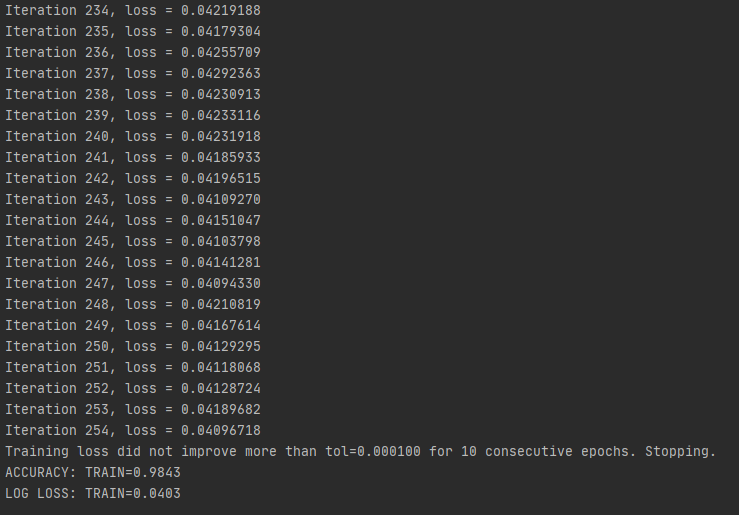
\includegraphics[width=140mm]{image/mlpresults2.png}
	\caption{Fase di addestramento e metriche risultanti.}
\end{figure}
Con questo modello si ha un accuracy pari a circa 0.98 e una log loss di circa 0.04.\\
Un altro tentativo è quello di inserire un ulteriore hidden layer di 100 neuroni sempre con funzione di attivazione lineare. Con tale modello si raggiunge la saturazione dell'addestramento (ovvero le 10 epoche consecutive dove il loss score non diminuisce di almeno $10^4$) molto prima (123 iterazioni) e si raggiunge un accuracy pari a circa 0.99 e una log loss pari a circa 0.03.\\
A questo punto si prova ad aggiungere un ulteriore hidden layer. In questo caso l'addestramento si conclude con 81 iterazioni, ma l'accuracy diminuisce a circa 0.98 e la log loss è pari a circa 0.03.\\
Si prova ora a cambiare la funzione di attivazione settandola come funzione sigmoide. In questo caso, anche con più hidden layer, si ha un accuracy pari a circa a 0.98 e una log loss a circa a 0.05.

\section{Conclusioni su MLP}
In base ai risultati ottenuti, per il dataset a disposizione, il modello con prestazioni migliori è senza dubbio il Multi-Layer Perceptron con due hidden layer di 100 neuroni l'uno e con funzione di attivazione lineare. Una limitazione, non poco importante, è il fatto che la fase di training può occupare molto tempo.
	\chapter*{Bibliografia}
	\begin{itemize}
		\item Machine Learning con Python: corso pratico di Profession AI 
		
		\href{https://www.udemy.com/course/machine-learning-pratico}{https://www.udemy.com/course/machine-learning-pratico}
		
		Corso di tutorial iniziale che mi ha fornito gli strumenti di base per svolgere il progetto.
		\item Documentazione di scikit-learn
		
		\href{https://scikit-learn.org/stable/index.html}{https://scikit-learn.org/stable/index.html}
		
		\item Slide del corso di Intelligenza Artificiale tenuto dal prof. Francesco Trovò
		
		\href{https://trovo.faculty.polimi.it/aibg_2018_2019.html}{https://trovo.faculty.polimi.it/aibg\_2018\_2019.html}
	\end{itemize}
\end{document}